\documentclass[12pt,fleqn]{article}
\usepackage{
  amsmath,
  booktabs,
  geometry,
  graphicx,
  microtype,
  parskip,
}
\usepackage[shortlabels]{enumitem}

\geometry{margin=3cm}

% equation line spacing
\setlength{\jot}{0.5cm}

% meta data
\newcommand{\chapter}{Chapter 1\--3}
\newcommand{\authorname}{Amo DelBello}
\newcommand{\classdescription}{MATH 1350-D2}
\newcommand{\classname}{Introduction to Statistics, Fall 2022}
\newcommand{\assignment}{\chapter\ In Class Exam}

\newcommand{\problem}[1]{\vspace{5ex}\section*{Problem \##1}}
\newcommand{\thead}[1]{\textnormal{\textbf{#1}}}
\newcommand{\tvspace}{\vspace{.25cm}}

\title{\classdescription\ \\ \classname\ \\ $\ $ \\ \assignment}
\author{\authorname}
\date{\today}


\begin{document}
\maketitle

\problem{1}
The sampling method appears to be flawed because it is a Convenience Sample. It was taken from a single group (members of a specific college). This group shares common interests and tendencies that may not be present, or may be present but to a greater or lesser degree, in the general population. Therefore, the conclusions reached in the study are not likely to be accurate.


\problem{2}
Correlation is not causation. Perhaps there are other factors in the lives of the piano playing students that contribute to higher math scores. The ability to pay for piano lessons indicates these students may be living in homes with higher income. The fact that they are involved in such activities indicates their care-givers take an interest in them and may indicate a tendency for a healthier home life. Perhaps an aptitude for piano causes an aptitude for math but I believe it is more likely that they are both a result of other external factors that contribute to and encourage learning in general.


\problem{3}
$(17 / 25) * 100 = 68$

\textbf{C:\ $68\%$}


\problem{4}
$115 * .41 = 47.15$

\textbf{A:\ 47}


\problem{5}
Temperature can be an infinite number of values.

\textbf{B:\ Continuous}\

\problem{6}
The values are just labels for categories

\textbf{D:\ Nominal}


\problem{7}
You can order ages. Ratios make sense \-- someone can be twice as old as someone else. There is a natural zero.

\textbf{A:\ Ratio}


\problem{8}
Nationalities are non-numerical data that cannot be ordered.

\textbf{D:\ Nominal}


\problem{9}
The sample is \textbf{50,000 randomly selected college students}. The population is \textbf{all college students}. Because the sample is so large and is randomized, it is \textbf{likely to be representative of the population}.


\problem{10}
Every 49th student is selected.

\textbf{D:\ Systematic}


\problem{11}
The population is subdivided into strata and then randomly selected within each strata.

\textbf{B:\ Stratified}


\problem{12}
The first 100 items are selected.

\textbf{D:\ Convenience}


\problem{13}
\textbf{D:\ No; no}


\problem{14}
\begin{tabular}{@{}ll@{}}
  \thead{Scores} & \thead{Relative Frequency} \\
  \toprule
  0\--60 & 10.34\% \\
  61\--70 & 34.48\% \\
  71\--80 & 37.93\% \\
  81\--90 & 13.79\% \\
  91\--100 & 3.45\% \\
  \bottomrule
\end{tabular}
\vspace{.25cm}

The correct values are listed in \textbf{Table B}.


\problem{15}
The center of the third class is $(120 + 130) / 2 = 125$.

\textbf{A:\ 125}


\problem{16}
\textbf{Yes}, the distribution appears to be normal.


\problem{17}
\textbf{C} appears to have the strongest linear correlation.


\pagebreak
\problem{18}

\begin{figure}[ht]
  \centering
  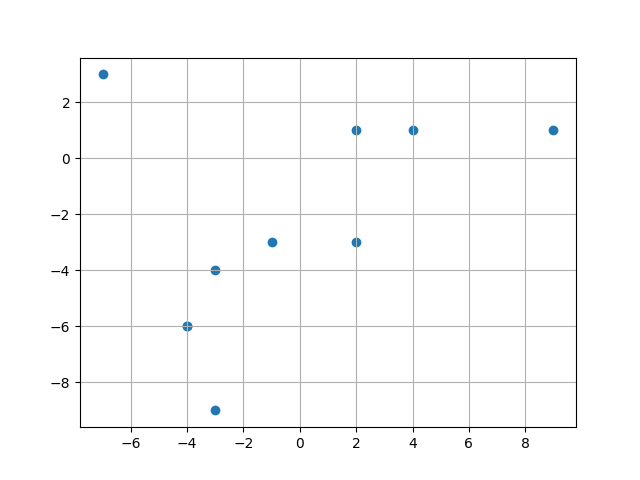
\includegraphics[width=12cm]{assets/scatter-plot.png}
\end{figure}

The correct scatterplot is shown in \textbf{Plot C}.

\problem{19}
The correct stemplot is shown in \textbf{Table B}.


\pagebreak
\problem{20}
\begin{figure}[ht]
  \centering
  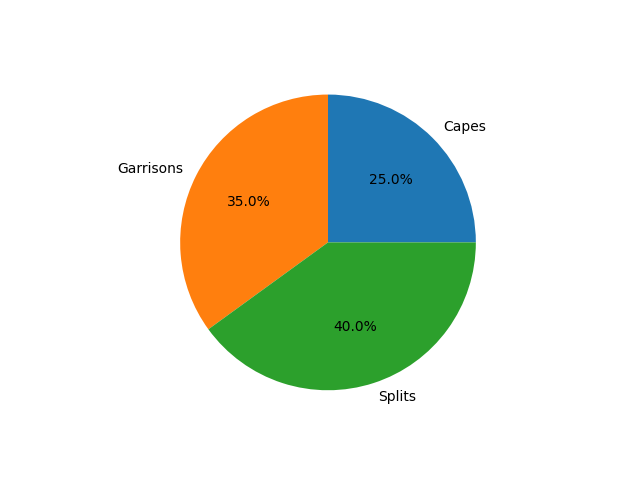
\includegraphics[width=12cm]{assets/houses.png}
\end{figure}

The correct pie chart is shown in \textbf{Chart B}.


\problem{21}
Yes the graph distorts the data. The y-axis (Number of accidents) does not start at zero. If I were to redesign the graph, I would make sure the y-axis started at zero.


\problem{22}
The graph is misleading because \textbf{both} the height and width of the television on the left are tripled to produce the television on the right. Instead of tripling the area of the television, it is cubed. This creates a visual impression that the television manufacturer's sales increased by much more than they actually did.


\problem{23}
\begin{equation*}
  \frac{(516 + 608 + 356 + 352 + 496 + 349 + 350 + 525 + 470 + 482)}{10} = 450.4
\end{equation*}
\textbf{C:\ 450.4}


\problem{24}
The values sorted are $[25, 25, 31, 53, 64, 73, 83]$

\textbf{C:\ $53^\circ F$}


\problem{25}
The values sorted are $[4.5, 4.5, 5.0, 5.0, 5.0, 5.8, 6.0, 6.2, 6.2, 6.2, 6.3, 6.5, 6.5, 6.6]$

\textbf{A:\ 5.0 oz, 6.2 oz}


\problem{26}
Weighted mean:
\begin{align*}
  \bar{x} &= \frac{\Sigma(w * x)}{\Sigma w} \\
  \bar{x} &= \frac{[(75 * .15) + (79 * .15) + (82 * .15) + (87 * .15) + (88 * .40)]}{(.15 + .15 + .15 + .15 + .40)} \\
  \bar{x} &= \frac{83.65}{1} \\
  \bar{x} &= 83.65
\end{align*}
\textbf{C:\ 83.7}


\problem{27}
The values sorted are $[1.5, 2.1, 3.5, 4.8, 5.6, 6.1]$ \\
$6.1 - 1.5 = 4.6$

\textbf{A:\ 4.6}


\problem{28}
\begin{align*}
  s &= \sqrt{\frac{n(\Sigma x^2) - (\Sigma x)^2}{n(n-1)}} \\
  s &= \sqrt{\frac{9(324 + 324 + 324 + 81 + 225 + 25 + 100 + 25 + 225) - (113)^2}{9(9-1)}} \\
  s &= \sqrt{\frac{14877 - 12769}{72}} \\
  s &= 5.41
\end{align*}
\textbf{B:\ 5.4}


\problem{29}
\begin{align*}
  z &= \frac{x - \bar{x}}{s} \\
  z &= \frac{96.7 - 98.20}{0.62} \\
  z &= -2.4
\end{align*}
\textbf{A:\ -2.4; unusual}


\problem{30}
\begin{align*}
  z &= \frac{x - \bar{x}}{s} \\
  z &= \frac{92 - 71}{15} \\
  z &= 1.4
\end{align*}

\begin{align*}
  z &= \frac{x - \bar{x}}{s} \\
  z &= \frac{688 - 493}{150} \\
  z &= 1.3
\end{align*}
\textbf{C:\ A score of 92}

\problem{31}
The minima and maxima of the two boxplots appear similar. The two boxplots have similar 3rd quartiles. The first quartile of the first boxplot is the same as the median of the second boxplot. In general, the values of the first boxplot seem greater than those in the second.


\problem{32}
\begin{figure}[ht]
  \centering
  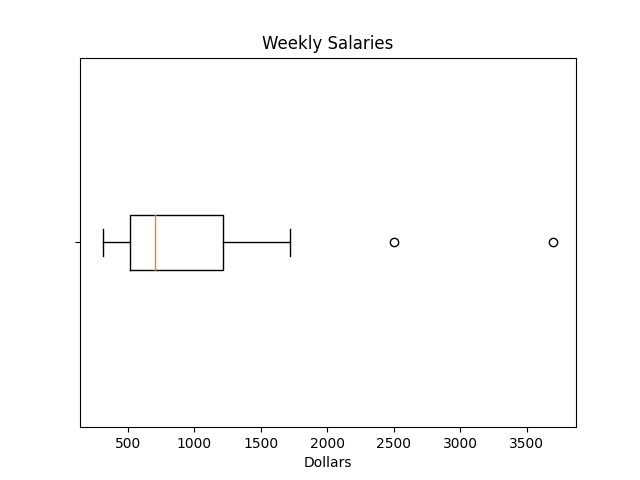
\includegraphics[width=12cm]{assets/weekly-salaries.png}
  \caption{Weekly Salaries}
\end{figure}
\textbf{StatCrunch 5-number summary}: $[310, 500, 700, 1250, 3700]$ \\
\textbf{matplotlib 5-number summary}: $[310, 515, 705, 1212.5, 3700]$ \\

I'm getting different values from matplotlib and statcrunch and neither align exactly with the options to chose. I think it's because of the way they are calculating outliers. The one that's closest is: \textbf{B}


\problem{33}
\textbf{Plot B} shows the strongest linear correlation.


\problem{34}
Correlation is not causation. The correlation could be explained by increases and decreases in the population overall. As the population increases in a town, both the number of movie theaters and the homicide rate will increase.


\end{document}
